\documentclass{tufte-handout}

\usepackage{ntheorem}
\usepackage{graphicx}
\usepackage{amsmath}
\usepackage{amssymb}
\usepackage{hyperref}
\usepackage{epigraph}
\usepackage{booktabs}
\theoremstyle{break}
% \usepackage[
% bibencoding=utf8,% .bib file encoding
% maxbibnames=3, % otherwise et al
% minbibnames=1, % otherwise et al
% backend=biber,%
% sortlocale=en_US,%
% style=apa,% or authoryear
% % apabackref=false, % backreferences
% natbib=true,% for citet/citep, but this is for backward compatibility
% uniquename=false,%
% url=true,%
% sortcites=false,
% doi=true,%
% eprint=true%
% ]{biblatex}
% \addbibresource{lecture_note_bib.bib}

\hypersetup{
  colorlinks,
  urlcolor = blue,
  pdfauthor={Paul Goldsmith-Pinkham}
  pdfkeywords={econometrics}
  pdftitle={Lecture Notes for Applied Empirical Methods}
  pdfpagemode=UseNone
}
\newtheorem{ruleN}{Rule}
\newtheorem{thmN}{Theorem}
\newtheorem{assN}{Assumption}
\newtheorem{defN}{Definition}
\newtheorem{exmp}{Example}
\newtheorem{cmt}{Comment}
\newtheorem{discussion}{Discussion Questions}
\newtheorem{proof}{Proof}

\newcommand{\continuation}{??}
\newtheorem*{excont}{Example \continuation}
\newenvironment{continueexample}[1]
 {\renewcommand{\continuation}{\ref{#1}}\excont[continued]}
 {\endexcont}
\newcommand{\bY}{\mathbf{Y}}
\newcommand{\bX}{\mathbf{X}}
\newcommand{\bD}{\mathbf{D}}
\newcommand{\E}{\mathbb{E}}

\newcommand\independent{\protect\mathpalette{\protect\independenT}{\perp}}
\def\independenT#1#2{\mathrel{\rlap{$#1#2$}\mkern2mu{#1#2}}}
\DeclareMathOperator{\Supp}{Supp}

\usepackage{cleveref}
\crefname{appsec}{appendix}{appendices}
\crefname{appsubsec}{appendix}{appendices}
\crefname{assumption}{assumption}{assumptions}
\crefname{equation}{equation}{equations}
\crefname{exmp}{example}{examples}
\crefname{assN}{assumption}{assumptions}
\crefname{cmt}{comment}{comments}
\crefname{defN}{definition}{definitions}

\usepackage[nolist]{acronym}
\begin{acronym}
  \acro{CI}{confidence interval}%
  \acro{OLS}{ordinary least squares}%
  \acro{CLT}{central limit theorem}%
  \acro{IV}{instrumental variables}%
  \acro{ATE}{average treatment effect}%
  \acro{RCT}{randomized control trial}%
  \acro{SUTVA}{stable unit treatment value assignment}
  \acro{VAM}{value-added model}%
  \acro{LAN}{locally asymptotically normal}%
  \acro{DiD}{difference-in-differences}%
  \acro{OVB}{omitted variables bias}
  \acro{FWL}{Frisch-Waugh-Lovell}
  \acro{DAG}{directed acyclic graph}
  \acro{PO}{potential outcomes}
\end{acronym}

\def\inprobHIGH{\,{\buildrel p \over \rightarrow}\,} 
\def\inprob{\,{\inprobHIGH}\,} 
\def\indistHIGH{\,{\buildrel d \over \rightarrow}\,} 
\def\indist{\,{\indistHIGH}\,}

\usepackage[many]{tcolorbox} 
\definecolor{main}{HTML}{5989cf}    % setting main color to be used
\definecolor{sub}{HTML}{cde4ff}     % setting sub color to be used
\definecolor{sub2}{HTML}{fde9ce}     % setting sub color to be used

\tcbset{
    sharp corners,
    colback = white,
    before skip = 0.2cm,    % add extra space before the box
    after skip = 0.5cm      % add extra space after the box
}                           % setting global options for tcolorbox

\newtcolorbox{boxD}{
    colback = sub, 
    colframe = main, 
    boxrule = 0pt, 
    toprule = 3pt, % top rule weight
    bottomrule = 3pt % bottom rule weight
}


\newtcolorbox{boxF}{
    colback = sub2,
    enhanced,
    boxrule = 1.5pt, 
    colframe = white, % making the base for dash line
    borderline = {1.5pt}{0pt}{main, dashed} % add "dashed" for dashed line
}

\newtcolorbox{boxK}{
    sharpish corners, % better drop shadow
    boxrule = 0pt,
    toprule = 4.5pt, % top rule weight
    enhanced,
    fuzzy shadow = {0pt}{-2pt}{-0.5pt}{0.5pt}{black!35} % {xshift}{yshift}{offset}{step}{options} 
}
\usepackage{colortbl}


\usepackage{tikz}
\usepackage{verbatim}
\usetikzlibrary{positioning}
\usetikzlibrary{snakes}
\usetikzlibrary{calc}
\usetikzlibrary{arrows}
\usetikzlibrary{decorations.markings}
\usetikzlibrary{shapes.misc}
\usetikzlibrary{matrix,shapes,arrows,fit,tikzmark}

\title{Lecture 4 - Interference, Spillovers and Dynamics}
\author{Paul Goldsmith-Pinkham}
\date{\today}


\begin{document}

\maketitle

This lecture note will discuss what it means to relax the following assumptions from the previous lecture:
\begin{enumerate}
        \item Binary scalar treatment
        \item Single time period (e.g. one treatment within the person)
        \item SUTVA -- Stable Unit Treatment Value Assignment
\end{enumerate}

\section{Multivalued treatments}
So far, our discussion of treatment effects has focused on single binary treatments. This made life very easy, but we have a lot of other more complex settings. We'll consider a few different cases. First, a multi-valued treatment. Then, we'll consider a continuous treatment. Finally, we'll consider an unordered multi-valued treatment.


\subsection{Discrete multi-valued treatment}
Let's start with a discrete, multi-valued treatment to start: $D_{i} \in \mathcal{D} = \{0,1, \ldots, d\}$. This captures a simple setting like ``what is the impact of 0, 1, 2, or 3 children on labor force participation?'' In this setting, we can easily shift the scale up and down (``what is the impact of 5, 10, 15, or 20 minutes on a task'') but the order and spacing may matter, depending on how we choose to parameterize and estimate the treatment effect.

In this setting, how should  we consider the treatment effects? First, what should we consider the ``control''? We could consider the control to be the lowest value of the treatment, but that depends a bit on the context. For example, if we are considering the impact of 0, 1, 2, or 3 children on labor force participation, we might consider the control to be 0 children. However, if we are considering the impact of 5, 10, 15, or 20 minutes on a task, we might consider the control to be whatever the status quo was.

Formally, we define the potential outcome for any $d \in \mathcal{D}$ as $Y_{i}(d)$, and we consider the individual and average treatment effect difference between $d$ and $d'$ as:

\begin{align*}
    \tau_{i}(d, d') &= Y_{i}(d) - Y_{i}(d')\\
    E(\tau_{i}(d, d')) &= E(Y_{i}(d) - Y_{i}(d')).
\end{align*}
If strong ignorability holds, then this is also identified by simply conditioning on each observed value:\footnote{The overlap condition in strong ignorability with multiple treatments is more complicated, but effectively entails that for any $\bX$, there are observations for every $d$ in $\mathcal{D}.$}
\begin{align*}
  E(\tau_{i}(d, d'))  &= E(Y_{i} | D_{i} = d) - E(Y_{i} | D_{i} = d').
\end{align*}

This type of estimation is non-parametric in nature: we've assumed no functional form between the treatment and the potential outcome. A consequence of that, just like in the case with many covariates $\bX$, is that it requires a lot more data to provide precise estimates. If we wanted to consider the CATE:
\begin{align*}
  E(\tau_{i}(d, d')| \bX = x)  &= E(Y_{i} | D_{i} = d, \bX = x) - E(Y_{i} | D_{i} = d', \bX = x),
\end{align*}
then we'll need to condition on treatment catgories within each cell, which can be very data hungry, and less precise. 

Often, instead of estimating the effect for every point separately, we will postulate a model for the potential outcomes: 
\begin{align*}
  Y_{i}(d) = Y_{i}(0) + \tau_{i} d.
\end{align*}
Notice that in this case, this implies that for all $d, d'$ pairs
\begin{align*}
  \tau_{i}(d, d') &= \tau_{i},
\end{align*}
which is the slope parameter. Hence, estimation can be made more precise by pooling all of these estimands together into a single estimand $E(\tau_{i})$.\footnote{Other, more flexible parametric forms for $Y_{i}(d)$ could be chosen as well. The insights will carry through so long as the functional form is finite-dimensional.}


\begin{figure*}
  \makebox[0.8\textwidth]{%
  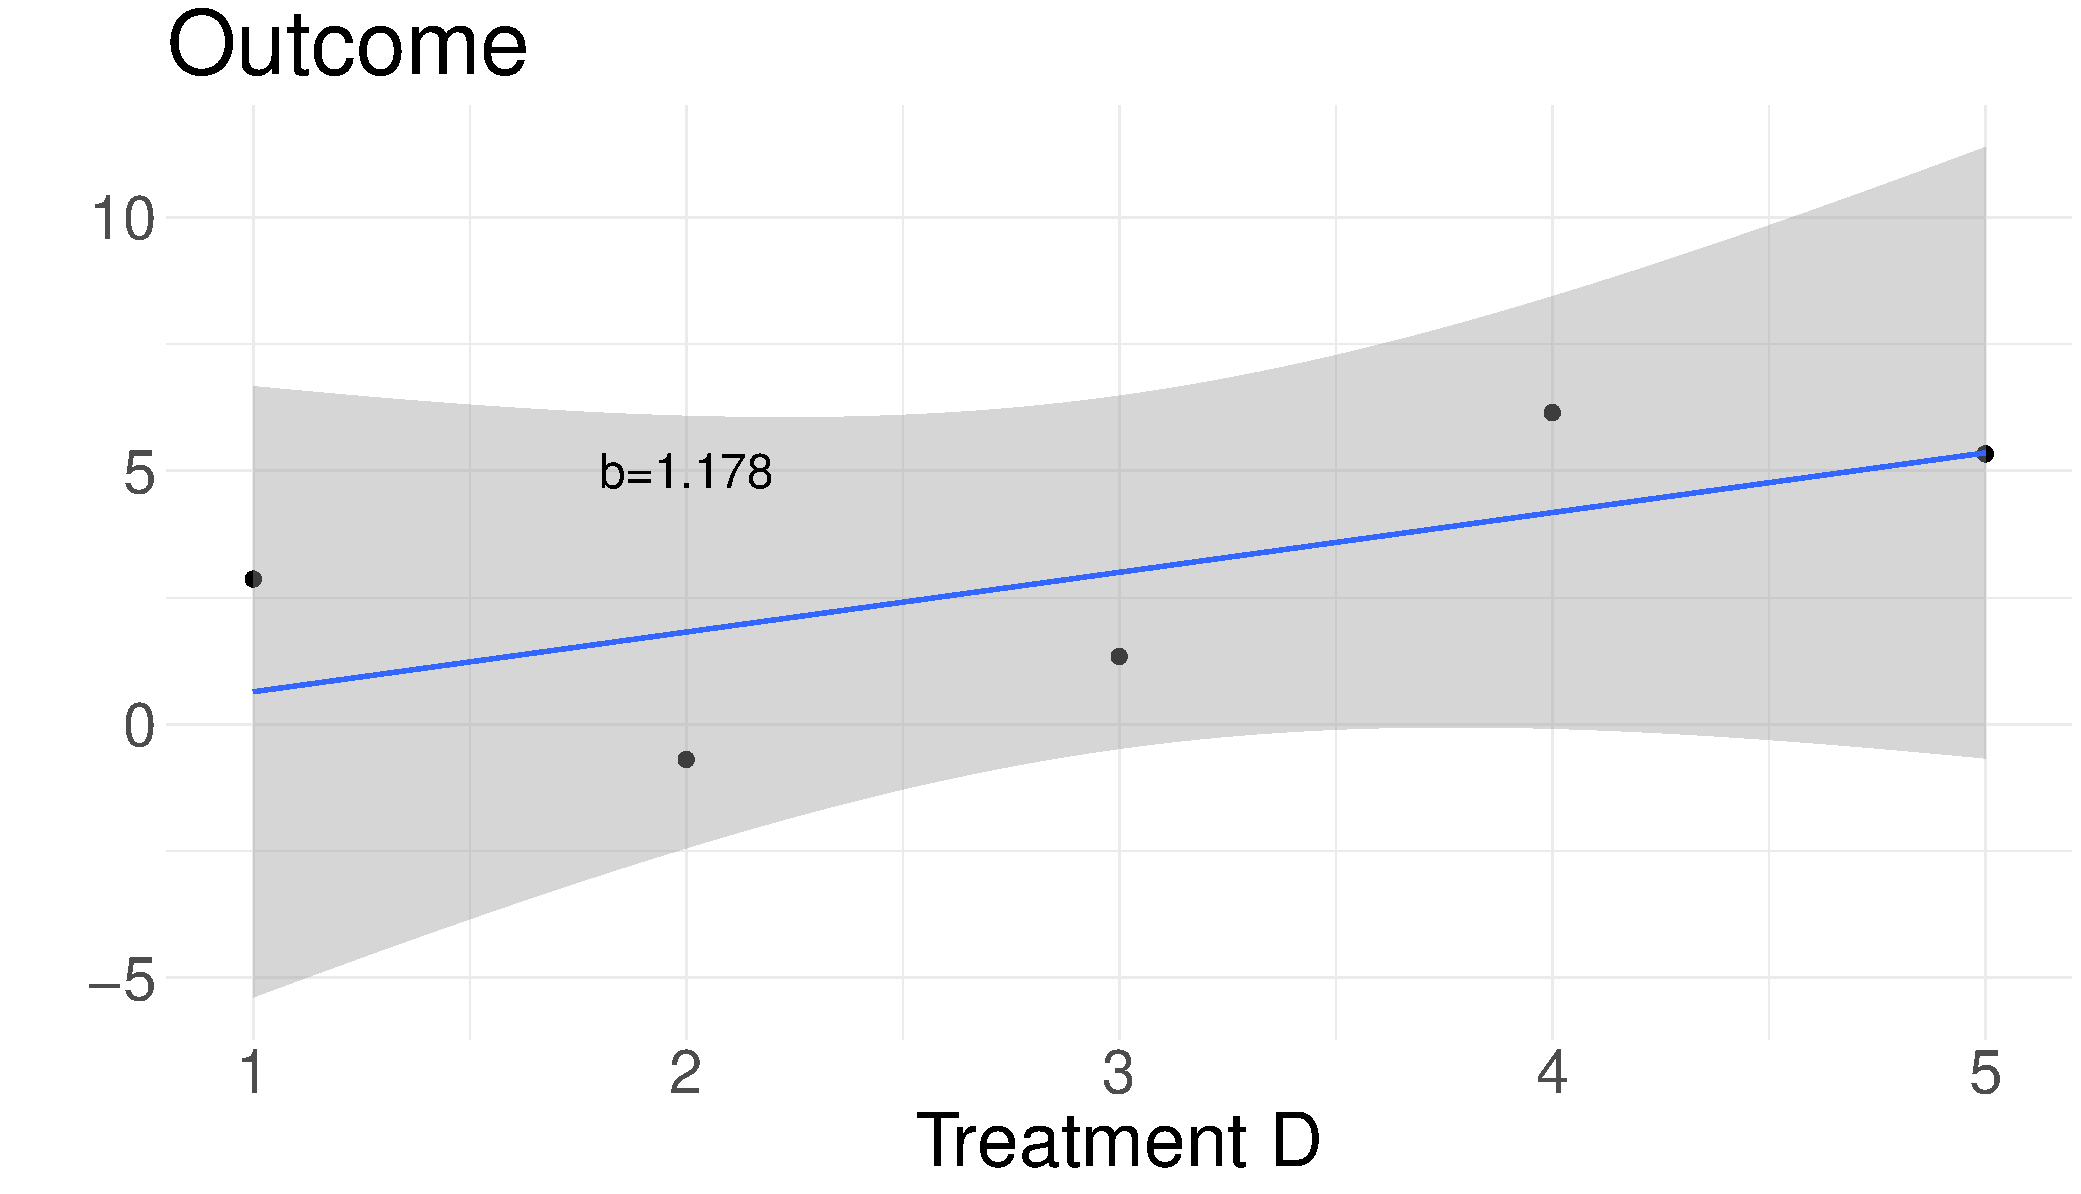
\includegraphics[width=\linewidth]{../lectures/images/linear_multivalued.pdf}}
  \caption{Linear effects estimated in simulated data with a true linear model for \Cref{exmp:linearmodel}}
  \label{fig:linearmodel1}
\end{figure*}

\begin{figure*}
  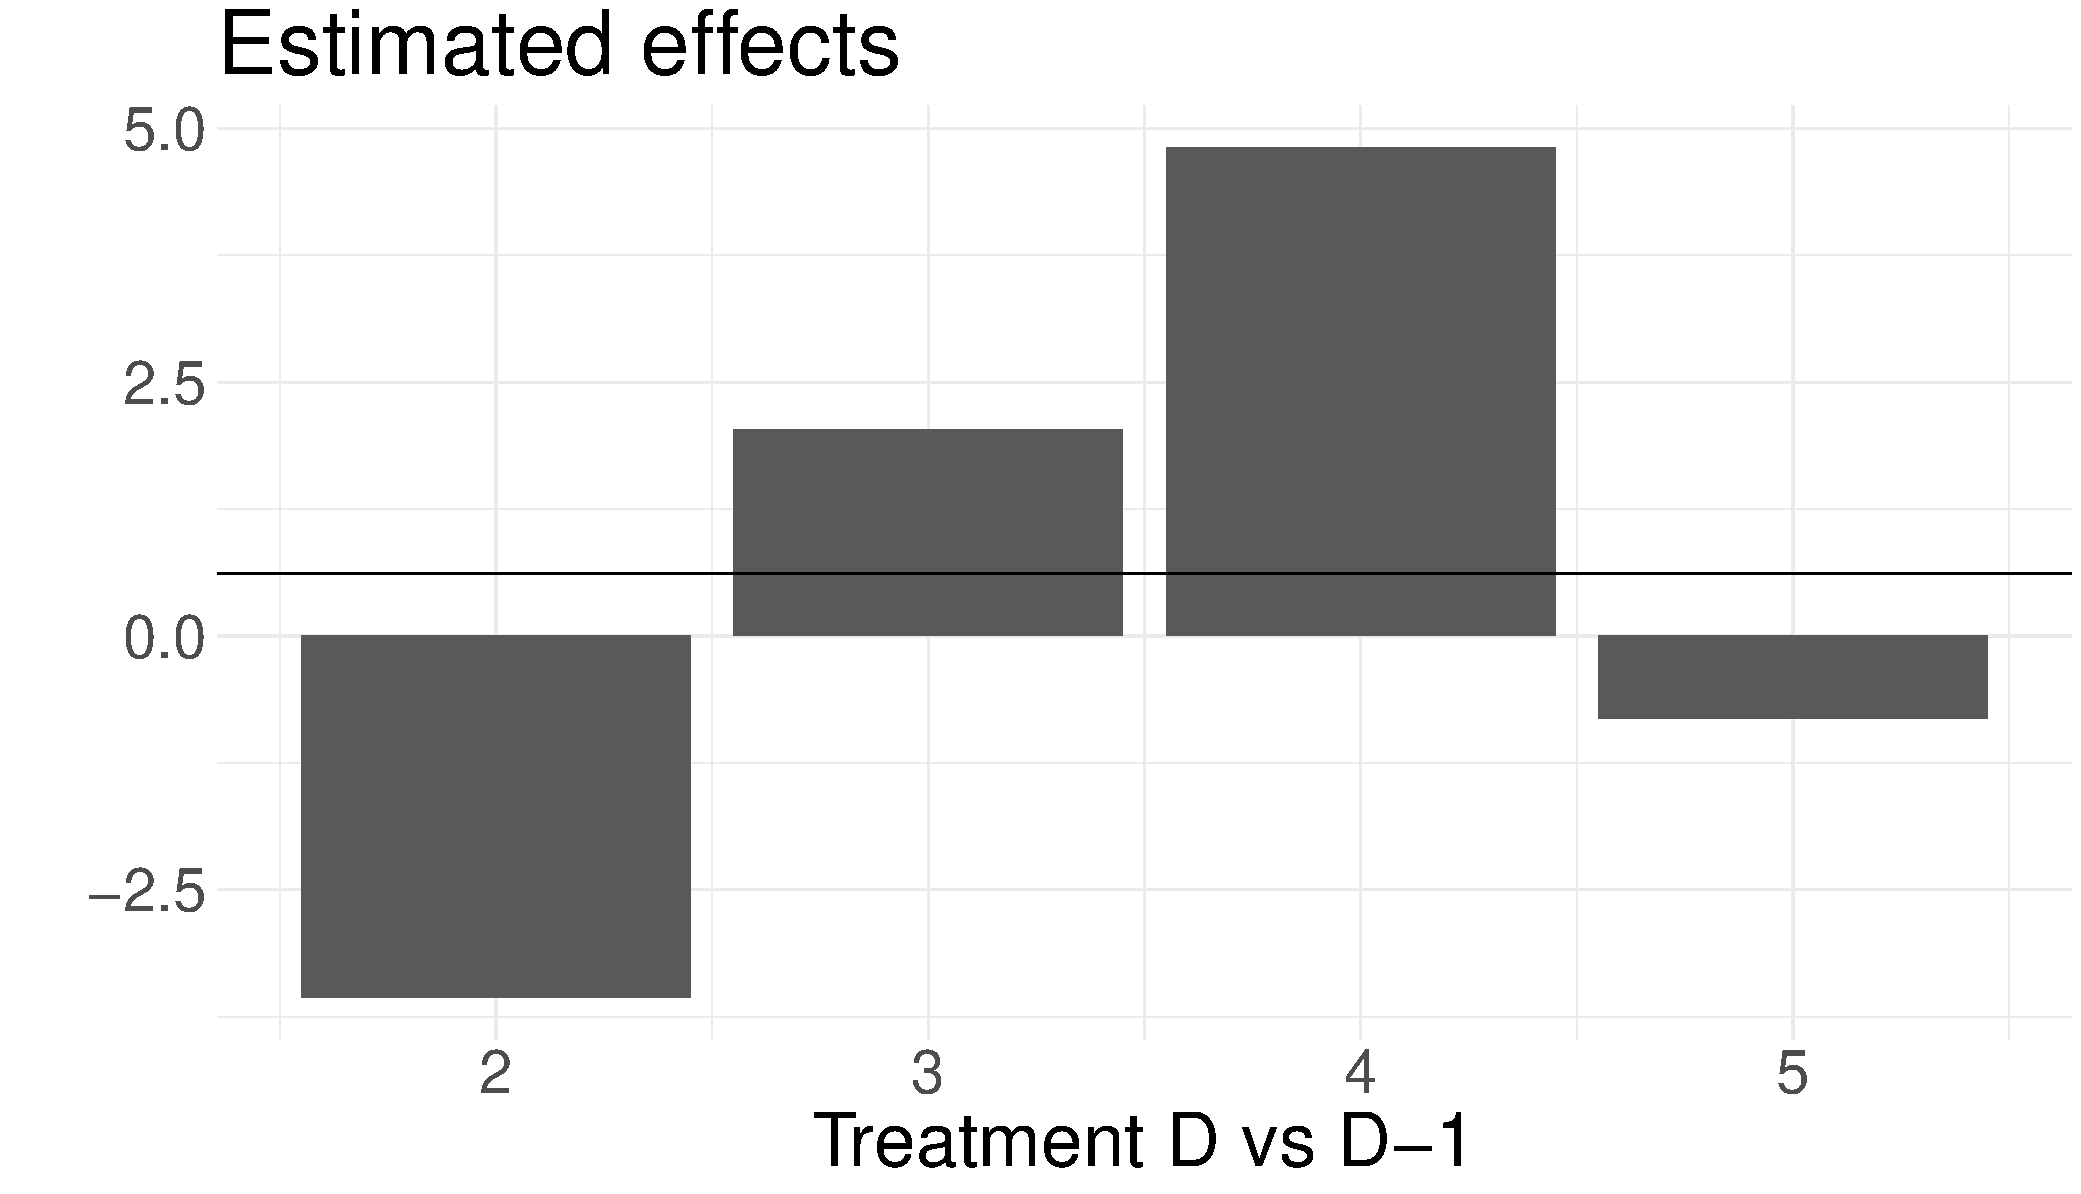
\includegraphics[width=0.8\linewidth]{../lectures/images/linear_multivalued2.pdf}
  \caption{Non-parametric effects estimated in simulated data with a true linear model for \Cref{exmp:linearmodel}}
  \label{fig:linearmodel2}
\end{figure*}
\begin{boxD}
  \begin{exmp}
    \label{exmp:linearmodel}
    Consider the following simulated data, where the true effect is linear and simulated such that $E(\tau_{i}(d, d') = d'-d$ and strong ignorability holds. 

    \hspace{10pt} Each dot in \Cref{fig:linearmodel1} is the estimated mean at the point, and we find a positive treatment effect. Imposing the model helps \emph{a lot} compared to non-parametric form. To see this, consider the treatment effect comparing $d$ to $d-1$ in \Cref{fig:linearmodel2}

    \hspace{10pt} The direction of the effect is much more ambiguous. This is a common tradeoff in estimation: imposing a model can help with precision, but can also lead to bias if the model is misspecified.
  \end{exmp}
  \end{boxD}


How should we consider these functional forms once we include controls? To see what I mean, consider the same context, but we now assume strong ignorability conditional on $\bX$. Then, we would need to estimate the slope $\tau_{i}$ for each value of $\bX$. How would that map over to a linear regression model? The simplest version would be one where the heterogeneity, $\tau_{i}$, is uncorrelated with $\bX$. Then, one way to estimate the ATE is to assume that $E(D_{i} | \bX) = \bX_{i}\beta$ (e.g. the propensity score is linear in $\bX$), we could estimate $E(\tau_{i})$ by simply running the following regression:

\begin{equation}
  \label{eq:covariate_linear}
  Y_{i} = \alpha + D_{i}\tau + \bX_{i} \beta + \epsilon_{i}
\end{equation}
and using $\tau$ as our estimate of $E(\tau_{i})$. But, if $\tau_{i}$ is not uncorrelated with $\bX$, then to estimate the ATE we would need to estimate the slope for each value of $\bX$, and pool separately. See \Cref{cmt:covariate_linear} for more details.

\begin{boxF}
\begin{cmt}
  \label{cmt:covariate_linear}
  It is worth thinking about why \Cref{eq:covariate_linear} will correctly estimate the ATE in this setting. To do this, let $E^{*}(D_{i} | \bX_{i})$ denote the best linear predictor of $D_{i}$ conditional on $\bX_{i}$. Now, note that by Frisch-Waugh-Lovell,
  \begin{equation}
    \tilde{Y}_{i} = \tilde{\alpha} + \tilde{D}_{i}\tau  + u_{i},
  \end{equation}
where $\tilde{Y}_{i} = Y_{i} - E^{*}(Y_{i}|\bX_{i})$ and $\tilde{D}_{i} = D_{i} - E^{*}(D_{i}|\bX_{i})$. Then,
\begin{align*}
  \tau &= \frac{E(\tilde{D}_{i}Y_{i})}{E(\tilde{D}_{i}^{2})}\\
   &= \frac{E(\tilde{D}_{i}Y_{i}(0))}{E(\tilde{D}_{i}^{2})} + \frac{E(\tilde{D}_{i}D_{i}\tau)}{E(\tilde{D}_{i}^{2})} 
\end{align*}
The first term is zero because the residual $\tilde{D}_{i}$ is mean independent of $\bX$ by the linearity of $E(D_{i}|\bX)$. Therefore, 
\begin{equation*}
  E(\tilde{D}_{i}Y_{i}(0)) = E(E(\tilde{D}_{i}Y_{i}(0)|\bX)) = E(E(\tilde{D}_{i}|\bX)E(Y_{i}(0)|\bX)) = 0.
\end{equation*}
Now note the second term by similar arugments:
\begin{equation*}
  \tau =  \frac{E(\tilde{D}_{i}D_{i}\tau)}{E(\tilde{D}_{i}^{2})} = \frac{E(Var(D_{i} | \bX)E(\tau|\bX))}{E(Var(D_{i} | \bX))}.
\end{equation*}
But, since we assumed $E(\tau|\bX) = E(\tau)$, this is just the ATE. If there is correlation of $\tau$ with $\bX$, we will get a different estimand.
\end{cmt}
\end{boxF}

\begin{boxK}
  \begin{discussion}
      Under what assumptions about $E(Y_{i}(0)|\bX_{i})$, instead of $E(D_{i}|\bX_{i})$, could we estimate the ATE using \Cref{eq:covariate_linear}? 
      \begin{enumerate}
        \item       Hint: think about a linear model for $E(Y_{i}(0))$ that is linear in $\bX_{i}$.\
        \item Second hint: the estimand could also be written as
  \begin{equation*}
  \tau = \frac{E(\tilde{D}_{i}\tilde{Y}_{i})}{E(\tilde{D}_{i}^{2})}
\end{equation*}    
    \end{enumerate}
  \end{discussion}
\end{boxK}

\subsection{Continuous valued treatment}
In many cases, the jump from discrete ordered treatments to continuous valued treatments is not large. Often, it just has to do with how many repeated observations we have of the same treatment; if each treatment value is unique, we're more likely to treat it as continuous. None of what we discussed above changes, except that direct non-parametric estimation becomes infeasible. 

Instead, to do non-parametric estimation we'll need to make other assumptions and use other methods, like kernel regression or local linear regression. We'll discuss these in future classes, but the key point is that we will want to make some amount of smoothness assumptions the effect of the treatment on the potential outcome.

Instead of non-parametric estimation, it is also reaosnable to assume a functional form, as above, and proceed from there. Then everything is exactly the same. 

\subsection{Unordered multi-valued treatment}
Finally, we might have a setting where the treatment is unordered. For example, we might consider the impact of different CEOs on firms' performance. In this case, we can't assume any particular ordering of the treatment, and it's not clear how to presume a functional form. Instead, there is a set of $K$ treatments in $\mathcal{D}$, and we can consider a set of different contrasts between them: $E(\tau_{i}(d, d'))$ for all $d, d' \in \mathcal{D}$.

A straightforward special case would be to consider a \emph{factorial} design: a randomized treatment where two treatments are cross-randomized, such that an individual can receive either no treatment, treatment 1, treatment 2, or both. Then, our potential outcomes look like \Cref{tab:factorial}. 

Given this, we have a number of potential estimands to consider. For example, we could consider the average treatment effect of treatment 1, but we would need to make a decision on what to do about the individuals who received both treatments. If the treatments interact in some way, then the average treatment effect of treatment 1 is not well-defined. Instead, we might consider the average treatment effect of treatment 1 for those who received treatment 2 ($E(Y_{i}(1,1) - Y_{i}(0,1))$), and the average treatment effect of treatment 1 for those who did not receive treatment 2 ($E(Y_{i}(1,0) - Y_{i}(0,0))$). 



\begin{table}[ht]
    \label{tab:factorial}
  \begin{center}
\begin{tabular}{c|rr}
  $ Y_{i}(\mathbf{D_{i}})$ & $D_{1i} = 0$ & $D_{1i} = 1$\\
  \midrule
  $D_{2i} = 0$ & $Y_{i}(0,0)$ & $Y_{i}(1,0)$\\
  $D_{2i} = 1$ & $Y_{i}(0,1)$ & $Y_{i}(1,1)$\\
\end{tabular}
\end{center}
\caption{Potential outcomes for a factorial design}
\end{table}

Of course, when data is sparse, we might want to do more with this, and just pool all of the data together: $E(Y_{i}(1, D_{i2}) - Y_{i}(0, D_{i2}))$. This is a reasonable estimand if we believe that the treatment effects are constant across the different levels of the other treatment, but if there are interactions, the external validity of this estimate will be suspect.\footnote{Think about why this is the case, if it's not clear.} See \citet{banerjee2021selecting} for a very interesting discussion on how to think about these types of estimands in the context of factorial designs when there are many treatments.

Factorial designs are the simplest case to consider, because the treatments are cross-randomized for many binary treatments. Often, we have just an ordered set of treatments. In this case, the same logic applies, but we have to be more careful about how we define the estimands. For example, if we consider the impact of different CEOs on firm performance, how do we define a ``control''? It is often not obvious, and we need to be careful about how we define the estimands. We may instead focus on the conditional means for each treatment, and then consider the full distribution of effects. This is the type of consideration in work thinking about place-based effects, for example, such as \citet{chetty2018impacts}.\footnote{It is interesting to think about these unordered treatments can sometimes be projected into continuous scalar measures. For example, when considering the impact of a CEO on a firm, you might measure a CEO's experience, and project the overall CEO's effect onto experience to capture a continuous measure of the CEO's effect. If you are additionally willing to assume that the effect of experience is the \emph{only} channel controlling the CEO's effect, then a more efficient procedure would use experience as the treatment effect, instead of the CEO. But that may not be a reasonable assumption. This issue arises when considering the effect of judges as in \citet{arnold2022measuring}.}

Estimating these effects seem like they should be straightforward extensions of the binary treatment case. However, the partial linear regression model fails us in this case. The variation in the propensity score across strata (controls) combined with heterogeneity in the treatment effects across strata will lead to contamination bias in the linear regression model. See \citet{goldsmith2022contamination} for more details, which we will revisit in the linear regression lectures.

Another issue that can arise is when the treatments are not cross-randomized, but instead are correlated on one another. A simple example of this is sequenced treatments: e.g. treatment 2 is only given after treatment 1, and only a subset of individuals receive treatment 1. See \Cref{fig:correlatedtreatment} for an example of this. In this case, it is not possible to identify the effect of $D_{2}$ separately from $D_{1}$: $E(Y_{i}(0,1) - Y_{i}(0,0))$ is not identified because $E(Y_{i}{(0,1)})$ is never observed. This rarely happens in many cross-sectional settings, but is quite common in dynamic settings (our next topic).
\begin{marginfigure}
  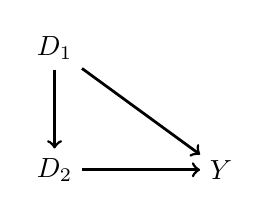
\begin{tikzpicture}
    % nodes %
    % \node[text centered] (z) {$Z$};
    \node[text centered] (t) {$D_{2}$};
    \node[right=1.5 of t, text centered] (y) {$Y$};
    \node[ above = 1 of t, text centered] (u) {$D_{1}$};

    % edges %
    % \draw[->, line width= 1] (z) --  (t);
    \draw [->, line width= 1] (t) -- (y);
    % \draw[->,red, line width= 1,dashed] (u) --node {X} (z);
    \draw[->,line width= 1] (u) --(t);
    \draw[->,line width= 1] (u) -- (y);
%\draw[->, red, line width=1,dashed] (z) to  [out=270,in=270, looseness=0.5] node{X} (y);
  \end{tikzpicture}
  \caption{Correlated treatments}
  \label{fig:correlatedtreatment}
\end{marginfigure}

\section{Treatment dynamics}
We will briefly discuss the impact of treatments over time to set the stage for our study of panel data later in the class. Consider a setting where we now observe $T$ time periods for a unit: $\bY_{i} = (Y_{i1}, Y_{i2}, \ldots, Y_{iT})$. Now, for each time period, there is a treatment $D_{it}$. It would be convenient to simply consider $Y_{it}(D_{it})$ as the potential outcome for an individual $i$ in period $t$, but that would be very restrictive: it would assume that only the period $t$ treatment affects the outcome in period $t$. A more general form would define a vector $\bD_{i} = (D_{i1}, D_{i2}, \ldots, D_{iT})$, and define the potential outcome in period $t$ as $Y_{it}(\bD_{i})$. In this case, however, we are perhaps too general: this allows for treatments in the future to affect current outcomes, which may be too strong.\footnote{This is often referred to as ``anticipatory effects'' in the literature.}

There are a large number of ways to simplify these potential outcomes. One simple way would be to restrict treatments to only affect outcomes in the future, and not the past. This is often referred to as the ``no anticipation'' assumption. The second is to assume that treatments will only turn on once: this allows the researcher to only consider the adoption date as the relevant period.\footnote{This is common in the staggered difference-in-difference setting.} 

As you can see, things become much more complex as soon as you allow for dynamic effects. In order to make progress, it will often be necessary to make restrictions on teh dynamics to make the estimands identified. We will discuss these in more detail when we discuss difference-in-differences.

\section{The SUTVA hits the fan}

In the discussion so far, the ``interference'' between treatments just comes from having multiple treatments to worry about, or from spillover across time. However, there are many other ways that treatments can interfere with one another. For example, what if treatments spill across units? What if the treatment of one unit affects the potential outcomes of another unit?

\begin{marginfigure}
  
  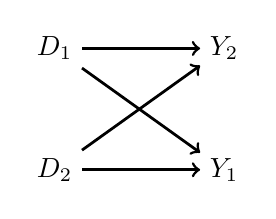
\begin{tikzpicture}
    % nodes %
    % \node[text centered] (z) {$Z$};
    \node[text centered] (t) {$D_{2}$};
    \node[right=1.5 of t, text centered] (y) {$Y_{1}$};
    \node[above=1 of y, text centered] (y2) {$Y_{2}$};        
    \node[ above = 1 of t, text centered] (u) {$D_{1}$};

    % edges %
    % \draw[->, line width= 1] (z) --  (t);
    \draw [->, line width= 1] (t) -- (y);
    \draw [->, line width= 1] (t) -- (y2);        
    % \draw[->,red, line width= 1,dashed] (u) --node {X} (z);
    \draw[->,line width= 1] (u) --(y2);        
    \draw[->,line width= 1] (u) -- (y);
%\draw[->, red, line width=1,dashed] (z) to  [out=270,in=270, looseness=0.5] node{X} (y);
  \end{tikzpicture}
  \caption{Interference between units}
  \label{fig:interference}
\end{marginfigure}
Recall the key assumption of Stable Unit Treatment Value Assumption (SUTVA): the potential outcomes of a unit do not vary with the treatment of other units. When could this be violated?

\begin{center}
    \textbf{\emph{So many places}}
\end{center}

Why does failure of SUTVA create an issue? Recall our discussion regarding marginal estimands when there were multiple treatments: even with random assignment, the estimates effect will be contaminated by others' treatment status, thereby leading to estimates that are not informative for the policy maker.

This type of problem is generally referred to as ``interference.'' It is challenging for identification, estimation and inference. For now, we'll focus on identification. I will flag three versions of this problem:        
      \begin{enumerate}
      \item Social interactons and peer effects
      \item Spatial spillovers
      \item Economic interactions -- budget constraints, etc.
      \end{enumerate}
 All these problems are versions of violation of SUTVA. With a clean, well-identified experiment, it is still possible to identify interesting estimands, but we may have to substantially modify our traditional estimators or make strong assumptions to make progress. One way to view this fact is that our original setting --- SUTVA, binary treatment and a single time period --- is a very special (and somewhat unrealistic) case.

\subsection{Social interactions and peer effects}
\begin{fullwidth}
\begin{quote}
  A variety of terms in common use connote endogenous social effects, wherein the
propensity of an individual to behave in some way varies with the prevalence of that
behaviour in some reference group containing the individual. These effects may, depending on the context, be called "social norms", "peer influences", "neighbourhood effects",
"conformity", "imitation", "contagion", "epidemics", "bandwagons", "herd behaviour",
"social interactions", or "interdependent preferences".
\end{quote}
--- \citet{manski1993identification}
\end{fullwidth}

Manski (1993) spawned a huge literature, much of which  focused on the linear-in-means model.\footnote{There are theoretical models microfounding a linear-in-means outcome model, which typically involve some kind of quadratic cost to deviating from the group. See \citet{shue2013executive} for an example}. An inherent issue, in my view, is that many empirical papers
jumped to this construction immediately. They did not have a structural interpretation in mind, but were instead interested in testing for the \emph{statistical} presence of spillovers across individuals. 

\begin{boxF}
  \begin{cmt}[Historical context on peer effects]
    \citet{manski1993identification} focused on a linear-in-means structural equation
  \begin{align*}
    Y &= \underbrace{\beta E(Y|g)}_{\text{endogeneous}} + \underbrace{\gamma_{1} E(X|g)}_{\text{exogeneous}} + \gamma_{2} X\\
    &+ \underbrace{\gamma_{3} g}_{\text{contextual}} + u. 
  \end{align*}
 Peers were not well-defined in the model, but empirically, were usually groups like
classrooms or clubs. What is important to note about this model is that it is a \emph{structural} model of the outcome, $Y$.  The reduced form is
\begin{align*}
  Y &=  \gamma_{1}/(1-\beta) E(X|g) + (\gamma_{2}/(1-\beta)) X\\
    &+ (\gamma_{3}/(1-\beta)) g + \tilde{u}, 
  \end{align*}
  which is estimable under special exogeneity assumptions on $X$, $g$ and $E(X|g)$. 

  \hspace{10pt} An innovation in this literature was to start using network data to define the group structure.  \citet{bramoulle2009identification} was a key paper in this literature, that reframed the Manski linear-in-means model to
  \begin{align*}
    Y &= \beta AY  + \gamma_{1} AX + \gamma_{2}X + \epsilon_{i},\; \\
    Y  &=   (I-\beta A)^{-1}\gamma_{1} AX + (I-\beta A)^{-1}\gamma_{2}X + (I-\beta A)^{-1}\epsilon_{i} \; 
  \end{align*}
where $A$ was an $n \times n$ matrix of individuals' connections. This was still a structural model, but allowed for richer data and more easily identified the effect of peers. 
\end{cmt}
\end{boxF}

Given that most researchers studying peer effects were not initially motivated by a structural model, it seems more natural to initially take a statistical approach to the problem. Namely, we would like to identify the effect of spillovers across units. How can we approach this problem using the tools we've developed so far?

Given $n$ individuals, for person $i$, how much interference can we allow? What types? 
    \begin{equation*}
      Y_{i}(D_{1}, D_{2}, \ldots, D_{n})
    \end{equation*}
    is far more extreme than
    \begin{equation*}
      Y_{i}(D_{i}, A\mathbf{D}_{n}).
    \end{equation*}
This question is analogous to our setting with treatment dynamics: how much spillover should we allow? SUTVA is complicated by the fact that there is no natural ``no anticipation'' condition due to the natural flow of time. As you might expect, there is no ``one solution'' in this setting. Certain restrictions need to be made to identify some estimands.

\citet{manski2013identification} is a very nice discussion of this in a \emph{very} high-level way. One key assumption he highlights is that ``anonymity'' of treatment spillover is a very important assumption. This implies that if I have peers who are treated, it does not matter \emph{which} of those peers are treated -- the impact on me is identical. This is a very strong assumption, but it is a necessary one to identify the effect of peers. If each peer's effect is allowed to be unique, then the effect of peers is not identified, since there is no way to separate out the treatment's spillover effect from the effect of the peer itself.\footnote{It might be doable in some networks, but it would be very challenging to do so, and require exogeneous network connections.}

A key question to keep in mind when considering spillovers: are you attempting to estimate the \emph{spillover} effect, or are you attempting to identify individual ATE in the presence of spillovers? These are very different estimands, and require different assumptions to identify. For the purposes of external validity, the latter is really only relevant if the context you apply the treatment in would have limited spillovers as well. 

We now briefly discuss two papers in this space to give intuition.

\paragraph{\citet{aronow2017estimating}} is a lynchpin paper in this setting that provides a framework for thinking about estimation and identification under general forms ofb interference. They use design-based inference, and consider the following generalized mapping.

\begin{defN}
  For any generalized vector of interventions, $\mathbf{D}_{n}$, there's an experimental design which assigns probabilities over $\mathbf{D}_{n}$. There is then an \emph{exposure} mapping $f(\mathbf{D}_{n}, \theta_{i})$ from these vectors to a treatment for an individual, which includes traits of an individual, $\theta_{i}$ (e.g. their network location) and the treatment vector, and maps it to an exposure outcome.
\end{defN}

This exposure mapping does two things. First, it makes restrictions on types of interactions (e.g. who can affect you and what type of effect it is).\footnote{Concretely: consider a network of peers affecting you. Is it the sum of your connected individuals in your network? Any exposure at all? Does it matter who in your network exposes you?} Second, it maps the experimental design to a propensity score of the exposure treatment. This allows the use of Horvitz-Thompson estimators.

So where are the bodies buried in this method? You have to have a correctly defined exposure mapping, and you have to have a correctly defined experimental design. In the case of a randomized experiemnt, the latter is straightforward, but the former is not, and typically needs to be motivated by theory, or asssessed for robustness. This is an active literature.

\paragraph{\citet{athey2018exact}} studies null hypothesis tests in networks under intereference. A key feature that this paper adds: testing specific types of analysis by creating ``artificial'' experiments. This paper is particularly powerful because it allows for testing in settings where there is uncertainty about the exposure mapping, and gives a framework for thinking about testing in a single network. 

\begin{boxF}
  \begin{cmt}
    When thinking about experiments in networks (and other settings), the structure of spillovers is very important. It is extraordinarily helpful to identify settings where there are \emph{zero} spillovers. Having units (such as villages, roommate pairs, etc.) that are isolated from one another is a very helpful way to identify the effect of the treatments. If we permute the treaments across these groups, then we can assess the spillover effects in a very clean way.
    
    \hspace{10pt}If, instead, we have only a single network, then we need to make strong assumptions about the structure of the network to identify the spillover effects. Namely, we need to have a well-defined exposure mapping that asserts that some units are sufficiently independent from others to serve as control units. 
  \end{cmt}
\end{boxF}

\begin{marginfigure}
  
\includegraphics[width=\linewidth]{../lectures/images/manskidrake.jpg}
  \caption{
    My views on social interactions summed up}
\end{marginfigure}

It is already very hard to do research on spillovers. Make sure to not ignore the difficult identification challenges and assumptions that you'll need to make.  If you need a model, that's great! But often you are just interested in starting from a statistical perspective, which suggests you shoudl focus on a design-based approach as in \citet{aronow2017estimating}.
 
\subsection{Spatial Spillovers}
Much of the spatial literature has sat in the same literature as social interactions. Distance on a network graph can be viewed as a similar distance metric to geographic (or economic) distance.Similar $A$ matrix, and consequentially similar structural models are proposed. 

The \citet{aronow2017estimating} setting allows for this as well.  From an identification standpoint, there isnothing deeply different here relative to networks, except that distance is potentially more continuous / complex. When we revisit simulated instruments, we will discuss some interesting implications raised by \citet{borusyak2020non}.

\subsection{Economic interactions}
Consider the following simple experiment -- I give one half of people in the economy checks for \$2000 dollars. I then study the impact of these checks on their consumption. Why might the effects be different than if I had run this experiment on a small share of individuals?

The economic spillovers coming through budget constraints are hugely important, but also deeply challenging as well. They require, often, modeling assumptions about spillovers. I will discuss two examples from the literature to give a flavor of the issues and solutions.

\paragraph{\citet{chodorow2019geographic}} studies the impact of fiscal stimulus on local employment. The key identification strategy is to use cross-region incidence of fiscal stimulus to identify multipliers on local employment. The paper argues that cross-region evidence bounds the estimand of interest, the impact of a \emph{national} stimulus, from below.

\begin{fullwidth}
  \begin{quote}
    Drawing on theoretical explorations, I argue that the typical empirical cross-sectional multiplier study provides a rough lower bound for a particular, policy-relevant type of national multiplier, the closed economy, no-monetary-policy-response, deficit-financed multiplier. The lower bound reflects the high openness of local regions, while the ``rough'' accounts for the small effects of outside financing common in cross-sectional studies.
  \end{quote}
\end{fullwidth}


\paragraph{\citet{sraer2023use}} use cross-firm experiment to influence the allocation of credit. Some firms got lots more credit! Some did not. How to aggregate up this affect? E.g. the policy effect is estimated by differencing the impact of the change on those who were more directly exposed vs. not -- however, this doesn't tell us about the aggregate impact on the economy. The paper argues, using economic theory, that these issues can be safely ignored under certain assumptions.

\begin{fullwidth}
  \begin{quote}
    Our paper bridges these two approaches. We offer a method to measure allocative efficiency in a (quasi-) experimental settings. This method works as follows. An econometrician observes firm-level data in an economy where a (quasi-) natural experiment has taken place. This experiment changes the set of frictions faced by treated firms while leaving control firms unaffected. Under the appropriate identifying assumption, the econometrician can estimate the causal effect of the experimenton firm-level outcomes, using classic difference-in-difference estimators. Standard policy evaluations typically estimate treatment effects on firm size or employment. However, these treatment effects alone cannot speak to allocative efficiency. To do so, we show that the econometrician needs to estimate treatment effects on the distribution of log marginal products of capital (lMRPKs). These estimates can then be injected in a simple aggregation formula to answer two simple questions: (i) how much did the actual policy change contribute to changes in aggregate efficiency (ex post evaluation)? (ii) how would aggregate efficiency have changed if the policy had been extended to all firms in the economy (scale-up)?
  \end{quote}
\end{fullwidth}


\bibliography{lecture_note_bib.bib}
\bibliographystyle{plainnat}

\end{document}